This section specifies the fiducial model, astrophysical parameters, tomographic redshift distributions, and reference data vectors used throughout the validation. The configuration follows the LSST DESC Science Requirements Document \citep[SRD;][]{2009arXiv0912.0201L} for a Y1 survey scenario with five lens and five source tomographic bins. We have verified that all results generalise to the Y10 survey scenario with ten lens bins; those results are not shown here for brevity.

\subsection{Fiducial cosmology} \label{sec:3.1}

The fiducial cosmology is a spatially flat \(\Lambda\)CDM model consistent with the \textit{Planck}~2018 constraints \citep{2020A&A...641A...6P}. The primary parameters are: \(\Omega_{\mathrm{m}} = 0.3152\), \(\Omega_{\mathrm{b}} = 0.0493\), \(\Omega_{\mathrm{CDM}} = 0.2645\), \(h = 0.6736\), \(n_{\mathrm{s}} = 0.9649\), \(A_{\mathrm{s}} = 2.083 \times 10^{-9}\), and \(\Omega_K = 0\). The dark-energy equation of state is fixed to the cosmological-constant values \(w_0 = -1\) and \(w_a = 0\). Neutrino masses are treated in a single-species approximation with \(\sum m_\nu = 0.06\,\mathrm{eV}\) and \(N_{\mathrm{eff}} = 3.033\). Linear transfer functions are computed with \texttt{CAMB} \citep{2000ApJ...538..473L}, and the non-linear matter power spectrum is obtained from the \texttt{HMCode2020} prescription \citep{2021MNRAS.502.1401M} with baryonic feedback parameterised by \(\log_{10}(T_{\mathrm{AGN}}/\mathrm{K}) = 7.8\).

\subsection{Astrophysical parameters} \label{sec:3.2}

The three classes of astrophysical bias defined in Table~\ref{tab:1} are specified as follows. The linear galaxy bias in the lens sample is modelled as
\begin{equation} \label{eq:3.1}
    b_{\mathrm{g}}(z) = \frac{b_\ast}{D(z)},
\end{equation}
where \(D(z)\) is the linear growth factor normalised to unity at \(z = 0\) and \(b_\ast = 1.05\) for the Y1 survey scenario \citep{2018PhR...733....1D}. This parameterisation ensures that the effective bias increases with redshift in a manner consistent with the evolution of dark-matter halo abundances, following conventions adopted in LSST DESC forecasts.

Galaxy shape alignments are described by the non-linear alignment (NLA) model \citep{2015PhR...558....1T, 2019PhRvD.100j3506B}. The alignment bias takes the form
\begin{equation} \label{eq:3.2}
    b_{\mathrm{I}}(z) = -\frac{C_1 \, \bar{\rho}_{\mathrm{m}}}{D(z)} \, A_{\mathrm{IA}} \left(\frac{1+z}{1+z_{\mathrm{pivot}}}\right)^{\eta_{\mathrm{IA}}},
\end{equation}
where \(C_1 = 5 \times 10^{-14}\,h^{-2}\,M_\odot^{-1}\,\mathrm{Mpc}^3\) is the normalisation constant, \(\bar{\rho}_{\mathrm{m}}\) the comoving mean matter density, and \(D(z)\) the linear growth factor. The fiducial values are \(A_{\mathrm{IA}} = 0.5\), \(\eta_{\mathrm{IA}} = 0\), and \(z_{\mathrm{pivot}} = 0.5\), applied uniformly across all source bins.

Lensing magnification is characterised by a per-bin constant response \(b_\mu^{(i)}\), determined by the slope of the cumulative galaxy number counts at the survey flux limit. For the five lens bins in the Y1 survey scenario, the fiducial values are
\begin{equation} \label{eq:3.3}
    b_\mu^{(i)} = \{0.659,\; 0.775,\; 0.815,\; 0.846,\; 0.994\}.
\end{equation}
All astrophysical bias parameters are held fixed throughout the validation and are not varied in the accuracy benchmarks. Figure~\ref{fig:1} illustrates the resulting tomographic redshift distributions for both the lens and source samples adopted in this work; the corresponding astrophysical bias values listed above are applied to these distributions when constructing the projected angular power spectra.

\subsection{Tomographic redshift distributions} \label{sec:3.3}

Tomographic redshift distributions are constructed following the LSST DESC SRD specifications using the \texttt{binny} package \citep{sarcevic2026binny}, which implements the underlying parametric forms and binning conventions adopted in the public \texttt{forecasting} analysis-choices repository. The underlying galaxy redshift distribution is described by a Smail-type parametric form,
\begin{equation} \label{eq:3.4}
    p(z) \propto \left(\frac{z}{z_\ast}\right)^{\beta} \exp\!\left[-\left(\frac{z}{z_\ast}\right)^{\alpha}\right],
\end{equation}
with shape parameters \((\beta, \alpha, z_\ast) = (2.0,\, 0.94,\, 0.26)\) for the lens sample and \((2.0,\, 0.78,\, 0.13)\) for the source sample. Photometric-redshift uncertainties are incorporated by convolving this distribution with a Gaussian error model characterised by a scatter of \(\sigma_z = 0.03\) for lens galaxies and \(\sigma_z = 0.05\) for source galaxies, with zero bias in both cases.

The convolved distribution is divided into \(N_\mathrm{B}\) tomographic bins per tracer sample as follows. In the Y1 survey scenario, \(N_\mathrm{B} = 5\) for both samples. Lens galaxies are assigned to five bins of equal redshift width \(0.2\) over the range \(0.2 \le z \le 1.2\). Source galaxies are partitioned into five bins of equal galaxy count. The resulting tomographic redshift distributions for both samples are shown in Figure~\ref{fig:1}. Each distribution is re-sampled onto a uniform redshift grid of \(N_\mathrm{Z} + 1 = 351\) points spanning \(0 \le z \le 3.5\) with a constant spacing of \(\Delta z = 0.01\), corresponding to \(N_\mathrm{Z} = 350\) redshift intervals. All distributions are normalised to unit integral. This grid defines the resolution at which the piecewise linearisation of physical quantities is performed in Section~\ref{sec:4}.

\begin{figure}[!htbp]
    \centering
    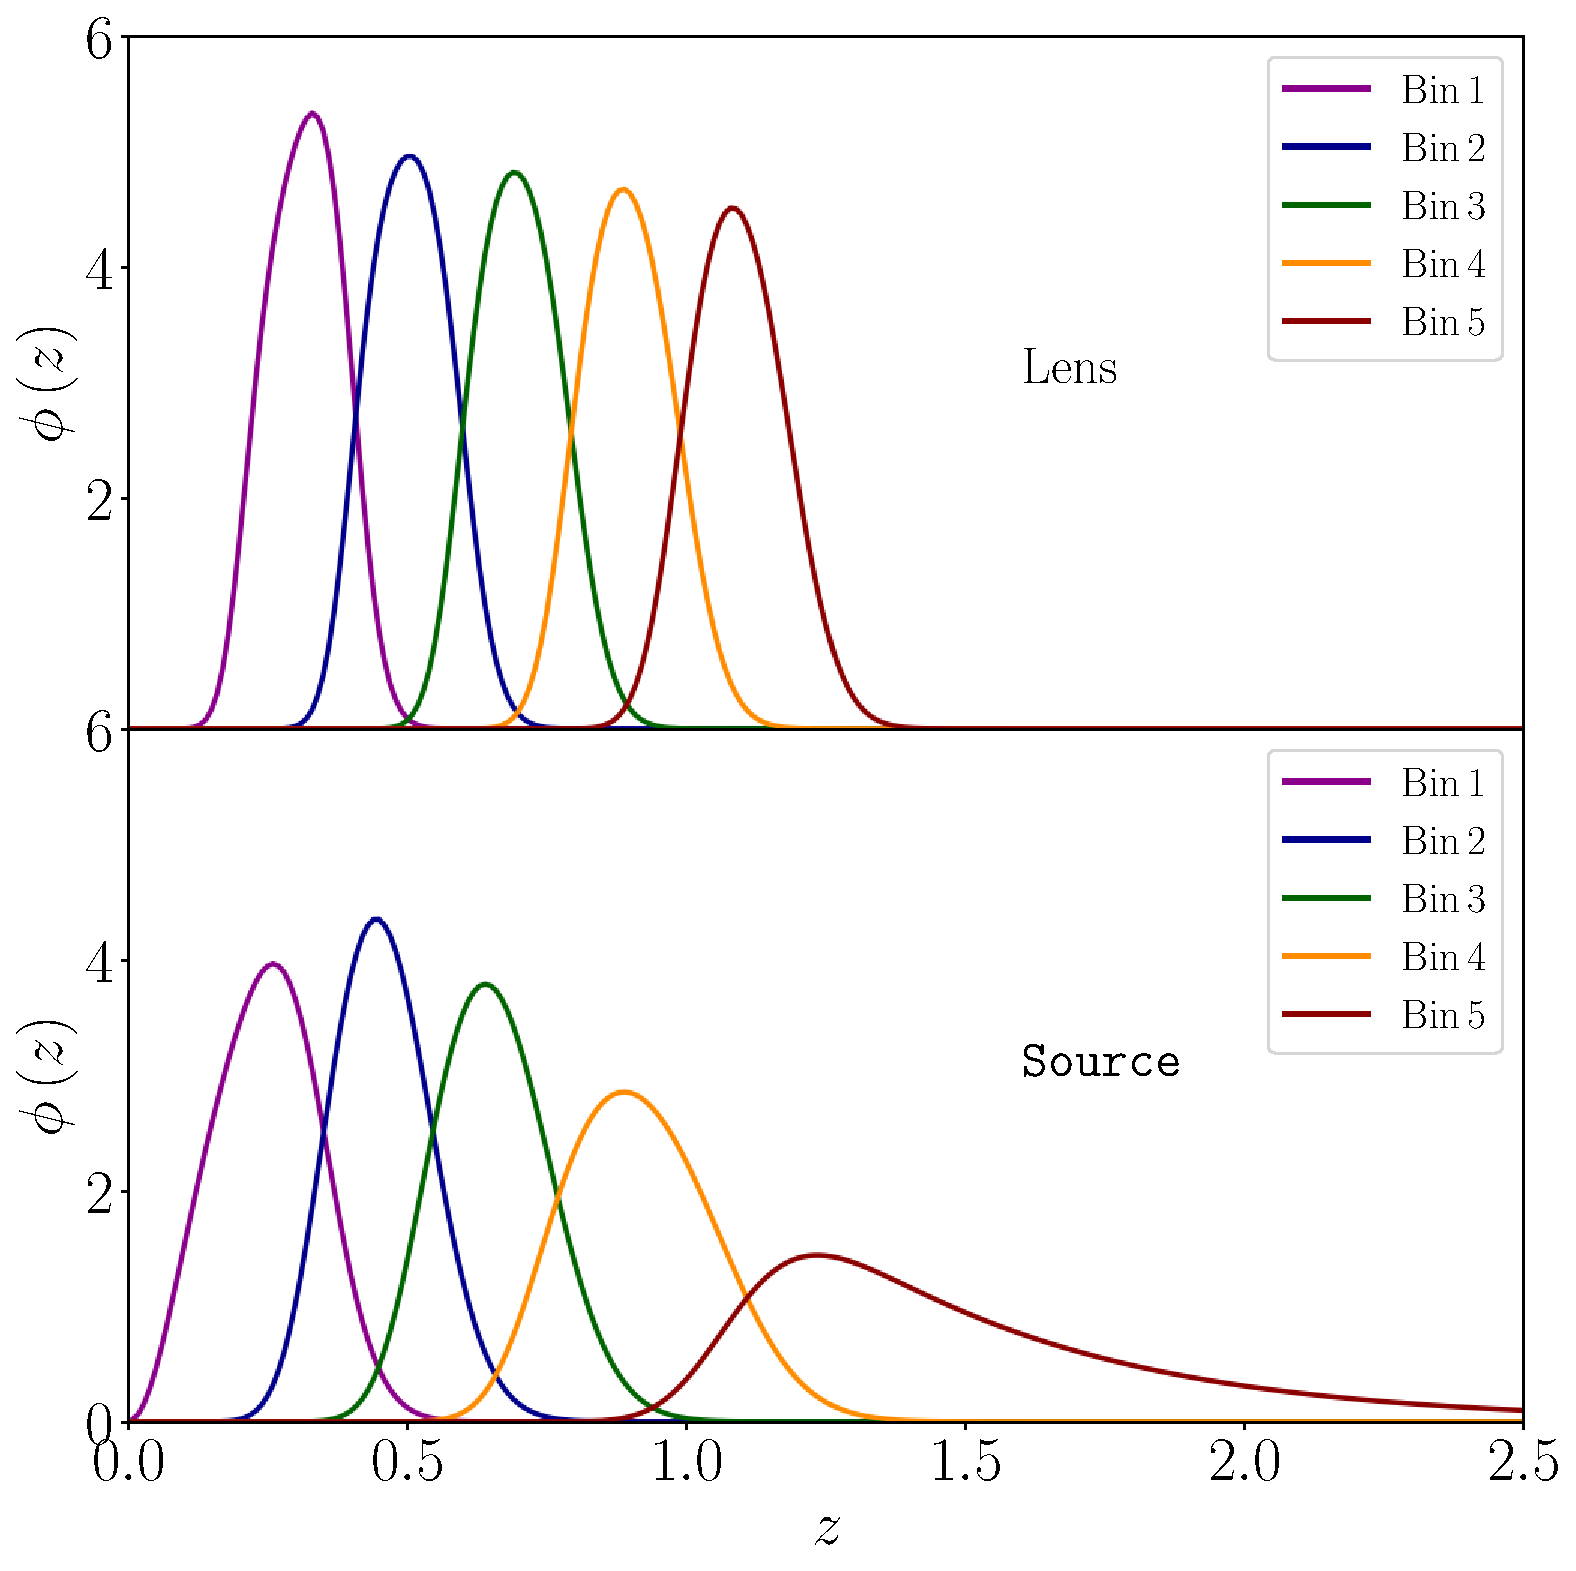
\includegraphics[width=\columnwidth]{figures/PSI_Y1.pdf}
    \caption{Tomographic redshift distributions for the LSST Y1 survey scenario. The upper panel shows the five equal-width lens bins over \(0.2 \le z \le 1.2\); the lower panel shows the five equal-count source bins. All distributions are normalised to unit integral.}
    \label{fig:1}
\end{figure}

The per-bin effective number densities, as adopted in the covariance calculation, are
\begin{equation} \label{eq:3.5}
    n_{\mathrm{eff}}^{\mathrm{lens}} = \{0.087,\, 0.096,\, 0.140,\, 0.181,\, 0.167\}\,\mathrm{arcmin}^{-2}
\end{equation}
for the five lens bins and
\begin{equation} \label{eq:3.6}
    n_{\mathrm{eff}}^{\mathrm{source}} = \{2.090,\, 2.298,\, 2.105,\, 1.901,\, 1.839\}\,\mathrm{arcmin}^{-2}
\end{equation}
for the five source bins.

The lens densities listed in Equation~\ref{eq:3.5} are deliberately lower than the SRD baseline of approximately \(18\,\mathrm{arcmin}^{-2}\) for the Y1 sample---roughly \(3.6\,\mathrm{arcmin}^{-2}\) per tomographic bin when divided evenly across the five lens bins---which counts all galaxies detected above the survey flux limit. A realistic \(3\times2\,\mathrm{pt}\) lens sample requires additional cuts on photometric-redshift quality, magnification response, and colour stability that reduce the usable density by an order of magnitude. We therefore adopt per-bin densities consistent with a DES-Y6-style lens selection \citep{2025arXiv250907964G} forward-modelled to LSST in \citet{Zhang.2026.DESC}. This bright-population definition is essential not only for representing realistic shot noise, but also for maintaining SRD-level photometric-redshift uncertainties on the lens redshift distributions: pushing to a fainter lens sample would dramatically inflate the photo-\(z\) calibration error budget and dominate over both the statistical and modelling uncertainties, providing a less realistic uncertainty baseline against which to validate the computational technique.

Source-sample densities, by contrast, are essentially unchanged from the SRD baseline, because source selection is dominated by shape-measurement quality cuts that do not differ substantially between the gold-detected and analysis-quality samples. We emphasise that this choice affects only the per-bin Gaussian covariance reference curves overlaid in Figures~\ref{fig:5}--\ref{fig:7}; the intrinsic accuracy of \texttt{LimberCloud} assessed in Section~\ref{sec:5} is independent of \(n_{\mathrm{eff}}\).

The per-component ellipticity dispersion is \(\sigma_\epsilon = 0.26\) in each source bin. The survey footprint covers \(18\,000\,\mathrm{deg}^2\), corresponding to a sky fraction of \(f_{\mathrm{sky}} \simeq 0.44\). Uncertainties in the tomographic redshift distributions are not varied in the present work; their treatment via analytic marginalisation is deferred to follow-up work.

\subsection{Angular power spectra and covariance matrices} \label{sec:3.4}

Reference angular power spectra serving as the validation benchmark are computed with \texttt{PyCCL} using the Limber approximation. The data vectors are evaluated at \(20\) logarithmically spaced multipole bins between \(\ell = 20\) and \(\ell = 2000\), where the effective multipole of each bin is taken as the geometric mean of its edges. The full \(3 \times 2\,\mathrm{pt}\) data vector comprises all unique tomographic auto- and cross-correlations for cosmic shear, galaxy--galaxy lensing, and galaxy clustering, including all contributions listed in Table~\ref{tab:1}.

Covariance matrices are computed with the \texttt{OneCovariance} code \citep{2025A&A...699A.124R}, which evaluates Gaussian, non-Gaussian (connected trispectrum), and super-sample covariance contributions using a halo-model framework. The input angular power spectra for the covariance calculation are evaluated at \(101\) logarithmically spaced multipoles over the same \(\ell\)-range, with \(20\) logarithmically spaced bins used for each of the lensing and clustering observables. The non-linear power spectrum within \texttt{OneCovariance} is computed using \texttt{HMCode2020} with the same baryonic-feedback parameter as above. The resulting covariance matrices provide a realistic, scale-dependent error budget that allows the accuracy of \texttt{LimberCloud} to be assessed against the expected statistical uncertainties of the survey.
